\capitulo{5}{Aspectos relevantes del desarrollo del proyecto}

\section{Introducción}

En este apartado explicamos el entrenamiento (\nameref{SectionEntrenamiento}) de nuestra red y las salidas que obtenemos. Comparamos los dos últimos modelos para ver cuál de ellos lo utilizamos para la aplicación de escritorio (\nameref{SectionComparacion}) y realizamos algunas pruebas al modelo seleccionado (\nameref{SectionPruebasModelo}).

También veremos las gráficas con los valores obtenidos tras el entrenamiento (\nameref{SectionGraficas}).

\subsection{Vocabulario}

Las palabras relacionadas con este apartado son:

\begin{itemize}
    \item \textbf{\textit{Steps}:} Un \textit{step} es un paso en el entrenamiento de la red neuronal. Tras finalizar un \textit{step} los datos de salida se utilizan para entrenar el siguiente.
    \item \textbf{\textit{Epochs}:} Son las etapas de nuestra red neuronal, por cada \textit{epoch} que se ejecuta se crea un modelo válido para  predecir defectos en nuevas imágenes. Una \textit{epoch} está formada por varios \textit{steps}, puedes asignar el número que mejor te convenga, en nuestro proyecto se ejecutan 500 \textit{steps} por \textit{epoch}.
    \item \textbf{\textit{Bounding Box}:} Cuadro delimitado donde se encuentran los defectos. Son cuatro valores que representan las coordenadas (\textit{x},\textit{y}) de las esquinas superior izquierda e inferior derecha del cuadro delimitador.
    \item \textbf{AP (\textit{Average Precision}):} Este término esta explicado en \ref{SectionAP}, el máximo que se puede obtener es de 1.
\end{itemize}

\section{Entrenamiento\label{SectionEntrenamiento}}

Para el entrenamiento de esta red se divide en tres etapas:

\begin{itemize}
    \item \textbf{Primera etapa:} Son 40 \textit{epochs} entrenando la cabecera de la red.
    \item \textbf{Segunda etapa:} Son 80 \textit{epochs} entrenando de la etapa 4 y superiores de la red.
    \item \textbf{Tercera etapa:} Son 40 \textit{epochs} entrenando todas las capas de la red.
\end{itemize}

\begin{figure}[h]
    \centering
    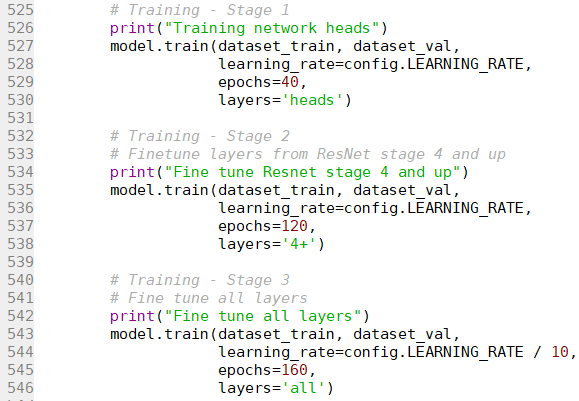
\includegraphics[width=0.63\textwidth]{codentrenamiento}
    \caption{Etapas de entrenamiento del código}
    \label{codentrenamiento}
\end{figure}

Esto es sólo una posible forma de entrenar la red (es la recomendada por Max Ferguson en su repositorio \cite{metal-defect-detection:repositorio}), hay más formas de entrenar la red, los parámetros para seleccionar que capas quieres entrenar son:

\begin{itemize}
    \item \textbf{heads:} Entrena la RPN, los clasificadores y los cabezales de máscara de la red.
    \item \textbf{all:} Todas las capas.
    \item \textbf{3+:} Entrena Resnet etapa 3 y superior.
    \item \textbf{4+:} Entrena Resnet etapa 4 y superior.
    \item \textbf{5+:} Entrena Resnet etapa 5 y superior.
    \item Una expresión regular para unir los nombres de las capas para entrenar.
\end{itemize}

Estas etapas están explicadas en \ref{resnetLabel}.

\begin{figure}[h]
	\centering
	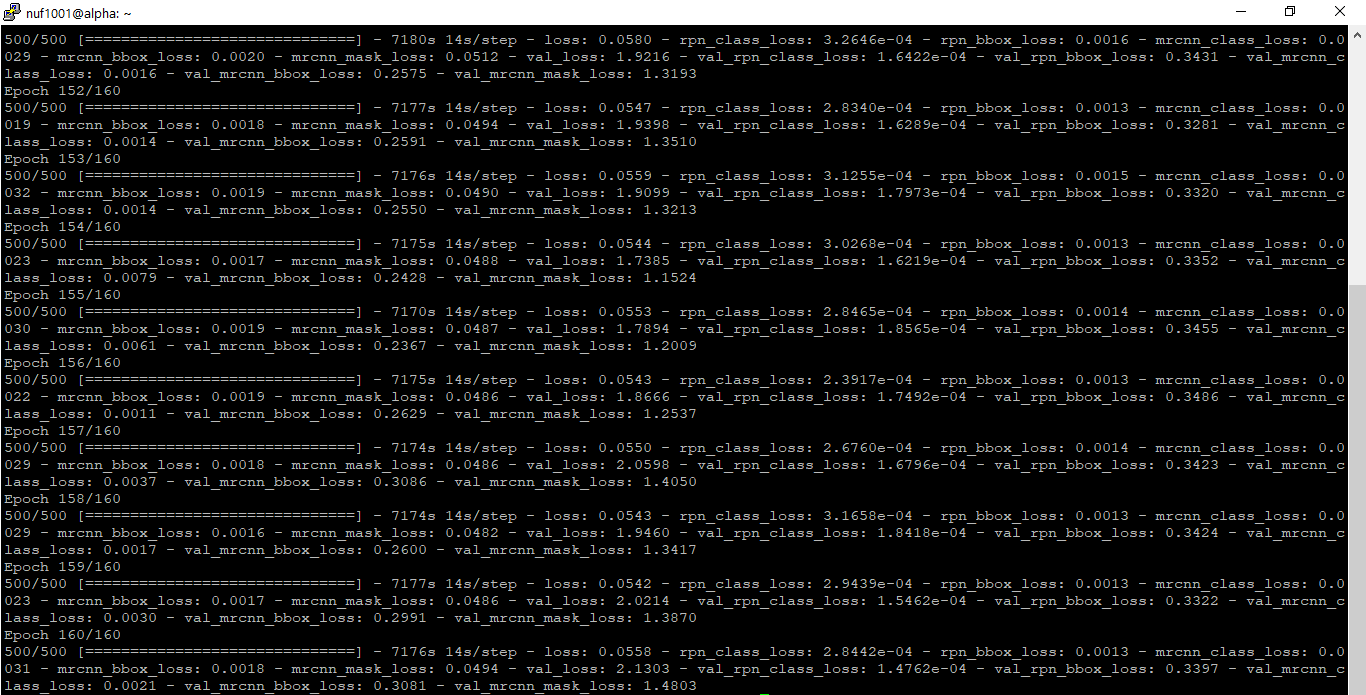
\includegraphics[width=1.3\textwidth]{entrenamiento160}
	\caption{Últimas \textit{epochs} del entrenamiento}
	\label{entrenamiento160}
\end{figure}

Se guarda un modelo por cada \textit{epoch}, es decir, al final del entrenamiento tendremos 160 modelos con 500 \textit{steps} por cada una, 80.000 \textit{steps} en total.

En la figura \ref{entrenamiento160} podemos ver la salida por pantalla del final del entrenamiento, las últimas 10 \textit{epochs} que se han realizado. Se va ha hacer incapié en las dos últimas \textit{epochs} la 159 y la 160 para saber cuál de los dos modelos es el mejor entrenado.

Los 5 \textit{losses} que vemos en la figura \ref{entrenamiento160} representan\label{losses}:

\begin{itemize}
    \item \textbf{rpn\_class\_loss:} Qué tan bien la red de propuestas de la región separa el fondo con los objetos, es decir, qué tan bien se diferencia el fondo (\textit{background} - BG) de los posibles defectos.
    \item \textbf{rpn\_bbox\_loss:} Qué tan bien los RPN localizan objetos.
    \item \textbf{mrcnn\_bbox\_loss:} Qué tan bien \textit{Mask RCNN} localiza objetos.
    \item \textbf{mrcnn\_class\_loss:} Qué tan bien \textit{Mask RCNN} reconoce cada clase de objeto.
    \item \textbf{mrcnn\_mask\_loss:} Qué tan bien \textit{Mask RCNN} segmenta los objetos.
\end{itemize}

Eso hace una mayor pérdida:

\begin{itemize}
    \item \textbf{\textit{loss}:} Una combinación de todos los \textit{losses} anteriores.
\end{itemize}

Todos estos \textit{losses} se calculan en el conjunto de datos de entrenamiento. Y los \textit{losses} para el conjunto de datos de validación son las que comienzan con ``val''.

\newpage

\subsection{Comparación modelos 159 y 160\label{SectionComparacion}}

\imagen{evaluate159_20}{Evaluación con el modelo número 159\label{evaluate159}}

\imagen{evaluate160_20}{Evaluación con el modelo número 160\label{evaluate160}}

Si comparamos los datos de la \textit{epoch} 160 y 159 que aparecen en las figuras \ref{entrenamiento160}, \ref{evaluate159} y \ref{evaluate160} vemos que la penúltima tiene mejores datos, es decir, el modelo 159 tiene un \textit{loss} menor que el modelo 160, ver en la tabla \ref{comparacionepochs}.

Como vemos en la tabla \ref{comparacionepochs} los datos los \textit{losses} de la \textit{epoch} 159 son mejores que los de la 160, pero vamos a hacer algunas pruebas para corroborarlo.

La diferencia de la mAP \cite{AP} que se observa en las figuras \ref{evaluate159} y \ref{evaluate160} no es muy grande, hay ocasiones en las que la evaluación del modelo 160 ha sido mejor que el del 159, pero predominan las pruebas con mejor AP en el modelo 159.

\newpage

\begin{table}[h]
	\begin{center}
		\begin{tabular}{l | c c c}
			Tipo de datos & \textit{Epoch} 159 & Comparación & \textit{Epoch} 160\\ \hline
			val\_loss & 2.0214 & < & 2.1303\\
			val\_rpn\_class\_loss & 1.5462e-04 & < & 1.4762e-04\\
			val\_rpn\_bbox\_loss & 0.3322 & < & 0.3397\\
			val\_mrcnn\_class\_loss & 0.0030 & > & 0.0021\\
			val\_mrcnn\_bbox\_loss & 0.2991 & < & 0.3081\\
			val\_mrcnn\_mask\_loss & 1.3870 & < & 1.4803\\
			mAP & 0.8583 & > & 0.8283\\
		\end{tabular}
		\caption{Comparación de las dos últimas \textit{epochs}}
		\label{comparacionepochs}
	\end{center}
\end{table}


\textbf{Imagen C0001\_0018:}

\imagen{img_C0001_0018_159}{Imagen C0001\_0018 con los \textit{Bounding Box} del modelo 159\label{img_C0001_0018_159}}

\imagen{tabla_C0001_0018_159}{Cuadrícula de la imagen C0001\_0018 de objetos de verdad y sus predicciones del modelo 159\label{tabla_C0001_0018_159}}

\imagen{img_C0001_0018_160}{Imagen C0001\_0018 con los \textit{Bounding Box} del modelo 160\label{img_C0001_0018_160}}

\imagen{tabla_C0001_0018_160}{Cuadrícula de la imagen C0001\_0018 de objetos de verdad y sus predicciones del modelo 160\label{tabla_C0001_0018_160}}

Las figuras \ref{img_C0001_0018_159} y \ref{img_C0001_0018_160} representa la imagen C0001\_0018 con los defectos detectados por los modelos 159 y 160 respectivamente. Las figuras \ref{tabla_C0001_0018_159} y \ref{tabla_C0001_0018_160} son las cuadriculas de los \textit{ground truth} y las predicciones hechas por los modelos entrenados. Las columnas representan los defectos reales que tiene la imagen y las filas los defectos detectados por el modelo, en este caso había tres defectos y los dos modelos han detectado los tres.

Con valores de la figura \ref{tabla_C0001_0018_159} vemos que el modelo 159 tiene una tasa de aciertos de un 98\% en el primer defecto, un 91.3\% en el segundo y un 94.6\% en el tercero (media de 94.63\%). Y en la figura \ref{tabla_C0001_0018_160} vemos que el modelo 160 tiene una tasa de aciertos de un 97.4\% para el primer defecto, un 94.6\% en el segundo y un 93.9\% en el tercero (media de 95.3\%). Estos valores son la coincidencia/superposición de las predicciones del modelo y del \textit{ground truth}. Salen de los decimales que aparecen en los cuadros de las figuras \ref{tabla_C0001_0018_159} y \ref{tabla_C0001_0018_160}.

 \textbf{Imagen C0001\_0004:}

\imagen{img_C0001_0004_159}{Imagen C0001\_0004 con los \textit{Bounding Box} del modelo 159\label{img_C0001_0004_159}}

\imagen{tabla_C0001_0004_159}{Cuadrícula de la imagen C0001\_0004 de objetos de verdad y sus predicciones del modelo 159\label{tabla_C0001_0004_159}}

\imagen{img_C0001_0004_160}{Imagen C0001\_0004 con los \textit{Bounding Box} del modelo 160\label{img_C0001_0004_160}}

\imagen{tabla_C0001_0004_160}{Cuadrícula de la imagen C0001\_0004 de objetos de verdad y sus predicciones del modelo 160\label{tabla_C0001_0004_160}}

Las figuras \ref{img_C0001_0004_159} y \ref{img_C0001_0004_160} representa la imagen C0001\_0004 con los defectos detectados por los modelos 159 y 160 respectivamente. Y las figuras \ref{tabla_C0001_0004_159} y \ref{tabla_C0001_0004_160} son las cuadriculas de los \textit{ground truth} y las predicciones hechas por los modelos entrenados. Las columnas representan los defectos reales que tiene la imagen y las filas los defectos detectados por el modelo, en este caso había dos defectos y el modelo 159 ha detectado tres y el modelo 160 cuatro.

Con valores de la figura \ref{tabla_C0001_0004_159} vemos que el modelo 159 tiene una tasa de aciertos de un 91.6\% en el primer defecto y un 93.3\% en el segundo (media de 61.63\%). Y en la figura \ref{tabla_C0001_0004_160} vemos que el modelo 160 tiene una tasa de aciertos de un 92.5\% para el primer defecto y un 93.3\% en el segundo (media de 46.45\%).

En esta imagen sólo hay dos defectos que son los que se encuentran en la parte inferior izquierda de la imagen. El modelo 159 ha detectado 3, el tercero lo ha detectado en el centro a la derecha, pero el modelo 160 ha detectado uno más en la parte inferior derecha. En estos dos errores vemos que no tienen asignado en un 1.000, esto indica que no es seguro al 100\% de que ahí se encuentre un error. Esto no indica que siempre que el valor no sea 1.000 no vaya a haber un error, sino que no que el programa no puede confirmar al 100\% que eso sea un defecto o parte de la imagen.

En conclusión, teniendo en cuenta los datos de la tabla \ref{comparacionepochs}, y la cantidad de defectos detectados por los modelos en la imagen C0001\_0004 (aunque los dos modelos han detectados defectos de más, el modelo 159 sólo ha detectado uno de más en cambio del modelo 160 han sido dos) he decidido seleccionar el modelo 159 para la app.

\subsection{Pruebas modelo 159 \label{SectionPruebasModelo}}

Evaluaremos la predicción de este modelo con tres pasos:

\begin{enumerate}
    \tightlist
    \item \textit{Region Proposal Network}.
    \begin{enumerate}
        \item Objetivos RPN.
    \end{enumerate}
    \item Clasificación de propuestas y detección.
    \begin{enumerate}
        \item Clasificación de propuestas.
        \item Detección paso a paso.
    \end{enumerate}
    \item Generación de máscaras.
    \begin{enumerate}
        \item Objetivos de las máscaras.
        \item Máscaras predichas.
    \end{enumerate}
\end{enumerate}

Añadiré un apartado con visualizaciones adicionales del mapa de funciones de la red troncal, los histogramas de \textit{bounding box} de el RPN y la distribución de las coordenadas \textit{y}, \textit{x} de las propuestas generadas.

Estas pruebas se realizarán con la última imagen mostrada en el apartado anterior, la figura \ref{img_C0001_0004_159}

\subsubsection{1. \textit{Region Proposal Network}\label{1_Region_Proposal_Network}}

El \textit{Region Proposal Network} (RPN) ejecuta un clasificador binario\footnote{En clasificador binario es el que podemos dividir en dos clases: “Positiva” y “Negativa”.} en muchos cuadros (anclas\footnote{Múltiples regiones posibles basadas en uniones espaciales de dimensiones fijas.}) sobre la imagen y devuelve puntuaciones de objeto/no objeto. Las anclas con un alto puntuación de ``objetividad'' (anclas positivas) se pasan a la etapa dos para su clasificación.

Cuando los anclajes positivos no cubren los objetos por completo el RPN también retrocede un refinamiento que se aplicará a los anclajes para cambiarlo y cambiar su tamaño un poco a los límites correctos del objeto.

\textbf{1.a Objetivos RPN\label{1_a_Objetivos_RPN}}

Los objetivos RPN son los valores de entrenamiento para el RPN. Para generar los objetivos, comenzamos con una cuadrícula de anclas que cubren la imagen completa a diferentes escalas, y luego calculamos la IoU de las anclas con el objeto de \textit{ground truth}. Los anclajes positivos son aquellos que tienen un \(IoU \geq\) 0.7 con cualquier objeto de verdad fundamental, y los anclajes negativos son aquellos que no cubren ningún objeto en más de 0.3 IoU. Las anclas intermedias (es decir, cubren un objeto por \( IoU \geq\) 0.3 pero \( < \) 0.7) se consideran neutrales y se excluyen del entrenamiento.

Para entrenar el RPN, también calculamos el cambio y el redimensionado necesarios para que el ancla cubra completamente el objeto de verdad del suelo.

\imagen{pruebas_1_a_1}{Imagen con anclajes positivos \label{pruebas_1_a_1}}

En la figura \ref{pruebas_1_a_1} se representan los anclajes positivos antes del refinamiento con la línea de puntos y los anclajes después del refinamiento con la línea sólida.

\subsubsection{2. Clasificación de propuestas y detección\label{2_Clasificación_de_propuestas_y_detección}}

Este paso se toman las propuestas de región de la RPN y se clasifican.

\textbf{2.a Clasificación de propuestas\label{2_a_Clasificación_de_propuestas}}

Ejecute los cabezales clasificadores en las propuestas para generar probabilidades de clase y regresiones de los \textit{bounding boxes}.

\imagen{pruebas_2_a_1}{Clasificación de propuestas \label{pruebas_2_a_1}}

\textbf{2.b Detección paso a paso\label{2_b_Detección_paso_a_paso}}

Mostraremos una muestra aleatoria de propuestas (200). Las propuestas clasificadas como \textit{background} están representadas con líneas de puntos, y el resto muestra su clase y puntuación de confianza de confianza.

En este caso tenemos 993 propuestas para \textit{Background} y 7 para \textit{Casting Defect}.

\imagen{pruebas_2_b_1}{ROI antes del refinamiento \label{pruebas_2_b_1}}

Ahora aplicamos el refinamiento del \textit{bounding boxes}. Ahora solo se visualizan las propuestas positivas.

\imagen{pruebas_2_b_2}{ROI depués del refinamiento \label{pruebas_2_b_2}}

Por último, se realiza una supresión no máxima (\textit{Non Max Suppression} - NMS) que es una técnica que filtra las propuestas en función de algunos criterios como la puntuación de confianza más alta o el IoU. Esto devuelve indicaciones de \textit{boxes} guardadas. Los \textit{boxes} que se devuelven son los que tienen un IoU por encima del umbral (el umbral es 0.3).

\imagen{pruebas_2_b_3}{Detecciones después de NMS \label{pruebas_2_b_3}}

\subsubsection{3. Generación de máscaras\label{3_Generar_máscaras}}

Esta etapa toma las detecciones (cuadros delimitadores refinados e ID de clase) de la capa anterior y ejecuta el cabezal de la máscara para generar máscaras de segmentación para cada instancia.

\textbf{3.a Objetivos de las máscaras\label{3_a_Objetivos_de_las_máscaras}}

Estos son los objetivos de entrenamiento para la rama de la máscara\footnote{El fondo es negro para que se va el contrate ya que casi toda la imagen es casi blanca.}.

\imagen{pruebas_3_a_1}{Objetivos de entrenamiento para la rama de la máscara \label{pruebas_3_a_1}}

\textbf{3.b Máscaras predichas\label{3_b_Máscaras_previstas}}

\imagen{pruebas_3_b_1}{Máscaras predichas\label{pruebas_3_b_1}}

\newpage

\subsection{Gráficas \label{SectionGraficas}}

Las gráfica \ref{grafica_loss} a \ref{grafica_rpn_class_loss}, que se muestran a continuación, representan la evolución de la figura de mérito de ``pérdida'' (\textit{loss}) en función del número de pasos (\textit{steps}). las variabes asociadas a estas gráficas están definidas en la Sección \ref{losses}.

\imagen{grafica_loss}{Gráfica del loss de las 160 \textit{epochs}\label{grafica_loss}}

\imagen{grafica_mrcnn_bbox_loss}{Gráfica del mrcnn bbox loss de las 160 \textit{epochs} \label{grafica_mrcnn_bbox_loss}}

\imagen{grafica_mrcnn_class_loss}{Gráfica del mrcnn class loss de las 160 \textit{epochs} \label{grafica_mrcnn_class_loss}}

\imagen{grafica_mrcnn_mask_loss}{Gráfica del mrcnn mask loss de las 160 \textit{epochs} \label{grafica_mrcnn_mask_loss}}

\imagen{grafica_rpn_bbox_loss}{Gráfica del rpn bbox loss de las 160 \textit{epochs} \label{grafica_rpn_bbox_loss}}

\imagen{grafica_rpn_class_loss}{Gráfica del rpn class loss de las 160 \textit{epochs} \label{grafica_rpn_class_loss}}

Los picos más significativos son los que salen cada 500 \textit{steps}. Ese es el momento en el que se termina un \textit{epoch} y empieza una nueva. Al principio hay una mejora bastante significativa en los datos, pero al final mejora más lentamente.

Para guardar estos datos he añadido en el archivo \texttt{generic\_utils.py} unas pocas líneas de código que me guardaban los valores en un archivo .csv. Este archivo se encuentra en \texttt{\textbackslash{}Anaconda3\textbackslash{}envs\textbackslash{}defect-detection\textbackslash{}Lib\textbackslash{} site-packages\textbackslash{}keras\textbackslash{}utils}.

\imagen{codigo_graficas}{Codigo para gradar los valores de las gráficas\label{codigo_graficas}}

Como vemos en la figura \ref{codigo_graficas} las líneas añadidas no cambian o modifican la funcionalidad del código. Este archivo no va a tener estas líneas, ya que es un archivo del entorno que se descarga en su creación.

